%!TEX program = xelatex
\documentclass[lang=cn,12pt]{elegantpaper}
\usepackage{adjustbox}
\title{A题}
\date{}

\setlength{\absleftindent}{0pt}
\setlength{\absrightindent}{0pt}

\begin{document}
	
\maketitle

\begin{abstract}
\noindent
\large
近年来,高送转通过除权等方式受到中小投资者的强烈追捧。因为实施高送转后股价将做除权处理,投资者可以通过填权行情从二级市场的股票增值中获利。很多股票在公布派送预案的第二天就直接涨停,但是等到除权后投资者再买入就会面临很大的回撤风险。如果我们能准确预测下一年可能实施高送转的上市公司并提前买入,这对我们投资的安全性具有很大的现实意义。基于此,我们将预测上市公司是否实施高送转为目标,将其划分为分类型预测,进而基于异种集成学习分类器的思想,使用硬投票器将  “决策树”  、“KNN算法” 和“ logistics回归 ” 组合起来,以达到预测准确率高的目的。在因子数据的选择中,我们把因子数据分为三类:基本因子、成长因子和潜在的因子,将原始数据中不相干数据和大面积缺失数据进行排除,提取出具有一定意义的因子数据,并且在后期训练模型中再次进行特征提取。以保证模型训练的有效性。此外,为了处理数据样本不平衡的情况,我们采用朴素随机过采样的方法,从少数类的样本中进行随机采样来增加新的样本,以提高模型预测的准确率。
\keywords{高送转,“决策树”,“KNN算法”,“ logistics回归”的异种集成学习,硬投票,朴素随机过采样}
\end{abstract}

\newpage
\tableofcontents
\newpage


\section{问题的提出}
\textbf{问题 1}:针对附件给出的因子数据,根据经济学意义以及数理统计方法,筛选出对上市 公司实施高送转方案有较大影响的因子。

在此问题中,我们借助现有的资料及论文和经济学原理,根据提供的原始数据样本,再进行包裹式的特征选择提取因子数据。

\textbf{问题 2}:利用问题 1 中确定的因子,建立模型来预测哪些上市公司可能会实施高送转, 并对附件提供的数据,用所建立的模型来预测第 8 年上市公司实施高送转的情况。 

在此问题中,我们会根据训练好的模型,预测第八年上市公司是否实施高送转,并在论文的最后列出。

\section{分析方法与过程}

\subsection{总体流程}

\begin{center}
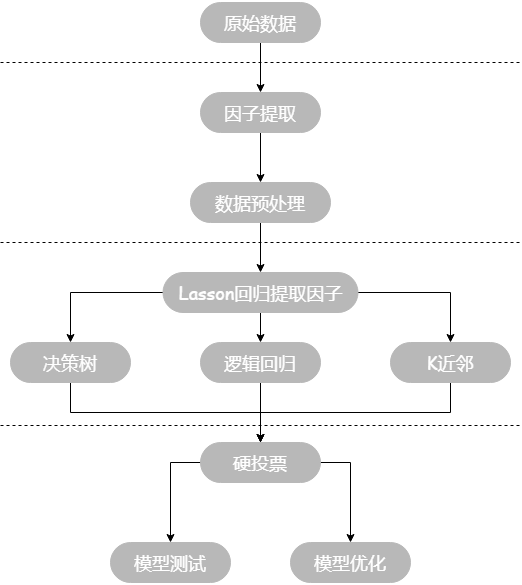
\includegraphics[scale=0.5]{1.png}
\end{center}


\textbf{步骤一}:获取分析的原始数据样本;

\textbf{步骤二}:数据分析,数据预处理,包括选取有用的因子数据,去除缺失值较多的因子;

\textbf{步骤三}:经过数据处理之后,用三种不同的分类算法进行建模和预测;

\textbf{步骤四}:运用硬投票,遵循“少数服从多数”原则预测第八年的高转送公司,再进行模型的测试和优化。

\subsection{具体步骤}

\subsubsection{数据分析}

\paragraph{数据的整体分析和介绍}:

1) 我们得到的原始数据分为三份,分别是年数据、日数据和基础数据。

2) 年数据里面包括各支股票的财务数据、每股股票数据和送转比例等数据,其中财务数据比较完整,一些上市较晚的公司的股票数据在未上市的年份缺失,我们将其视为异常值;日数据里包括每日股票的价格变动、财务数据和股票风险估计等数据,其中每股收益、每股净资产和每股资本公积金等数据在一段时间内无波动,并且某些股票的数据有缺失;基础数据里包括股票所属上市公司的上市年限和概念股板块。

\paragraph{选取基本因子、成长因子和可能潜在的因子,并说明原因}
:

1) 根据资料(论文标签)、经济学方面的知识和题目,我们确定因子分为基础因子(括股价、总股本、上市年限)、成长因子(每股未分配利润、每股资本公积、每股现金流量净额、每股收益、每股净资产、营业总收入同必增长)和潜在因子(次新股、预增预减、超涨超跌、近两年送转比率)。

2) 基本因子:根据经济学相关知识,高送转的目的之一是为了增加股票的流通性,股价越高,会使得股票流通性较差,而高送转可以帮助股票的价格大幅度降低以达到增加流通性的目的;股本小的个股通过高送转扩大股本欲望较高;\cite{基于模式识别的“高送转”预测模型}结论显示上市年限对高送转具有显著的负作用;

3) 成长因子:转增股本主要是将企业资本公积转入股本账户,送股实质上是将企业的留存收益转入股本账户,其中主要是将留存收益中的未分配利润部分送股,所以每股资本公积和每股未分配利润更大,企业高送转的可能性更高。营业总收入同必增长反映了上市公司的营业收入情况。每股现金流量净额、每股收益、每股净资产均反映了上市公司的财务情况。

4) 潜在因子:\cite{基于集成学习的上市公司高送转预测模型及投资策略设计}次新股高送转潜力更大。由于新上市企业在发行新股时都得了较高的股票溢价收入,因此尽管次新股可分配的利润可能不多,但由于有较高的资本公积,因此次新股的高送转比例更高。预增或预减可以作为上市公司营业状态的一个指标,而超涨超跌是股票价格异常的一个指标。近两年送转比率高的股票会更倾向于高送转。

\newpage
\paragraph{定义因子的具体处理方式}
:

1) 以年为单位提取因子数据,用K年的数据预测K+1的数据,即基于K年因子数据在K+1年实施的高送转行为定义为K+1年高送转。\cite{基于模式识别的“高送转”预测模型}

2) 基础因子中,选取每年十二月收盘价平均值作为K年的股价,总股本选取年数据中“实收资本(或股本)”作为标准,上市年限依据基础数据算出。日数据和年数据基本都有包含成长因子,但是日数据缺失值过多,因此选择年数据为标准,其中将“每股未分配利润+每股资本公积”作为一个因子数据。潜在因子均在基本数据中的概念板块中提取。将次新股、预增、超涨用1定义,非次新股定义为0,预减和超跌定义为-1。

3)表格:关键词的权重

\begin{center}
\begin{tabular}{|c|c|}
	\hline
	tag & weight \\\hline
	超涨  & 0.219  \\\hline
	预增  & 0.193  \\\hline
	预减  & 0.096  \\\hline
	次新股 & 0.086 \\\hline
\end{tabular}
\end{center}

\paragraph{计算各个因子的相关性和方差}
:

1. 方差

\begin{center}
	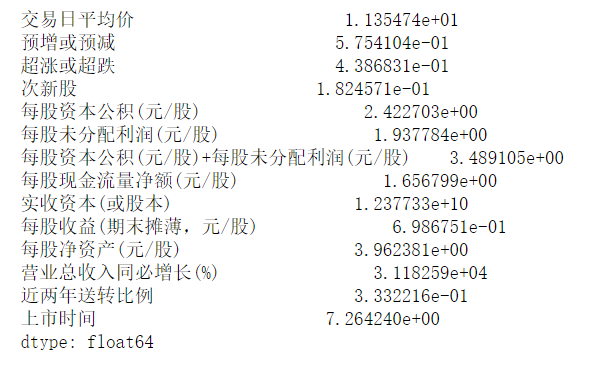
\includegraphics[scale=0.6]{2.png}
\end{center}

\newpage

2. 用皮尔森系数计算各个因子的相关性

\begin{center}
	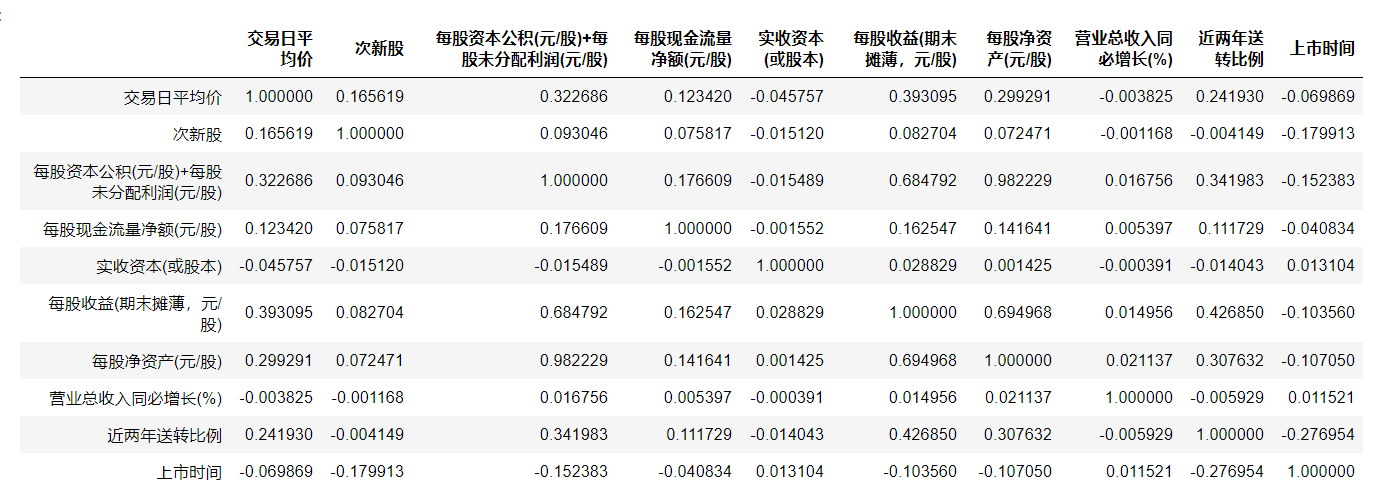
\includegraphics[width=1\columnwidth]{3.png}
\end{center}



\subsubsection{数据预处理}

\paragraph{因子定义}
:

\begin{center}
		\begin{tabular}{|l|l|l|l|}
			\hline
			因子类型 & 名称                                                                 & 说明                                                                        \\ \hline
			因变量  & 是否高送转                                                               & \begin{tabular}[c]{@{}l@{}}0为不发生高送转,\\ 1为发生高送转\end{tabular}   \\ \hline
			自变量  & \begin{tabular}[c]{@{}l@{}}每股资本公积(元/股)+\\ 每股未分配利润(元/股)\end{tabular} & 年数据                                                           \\ \hline
			& 每股现金流量净额(元/股)                                                       & 年数据                                                            \\ \hline
			& 每股收益(期末摊薄,元/股)                                                      & 年数据                                                             \\ \hline
			& 每股净资产(元/股)                                                          & 年数据                                                            \\ \hline
			& 实收资本(或股本)                                                           & 年数据                                                            \\ \hline
			& 营业总收入同必增长(\%)                                                       & 年数据                                                             \\ \hline
			& 交易日平均价                                                              & \begin{tabular}[c]{@{}l@{}}以每年12月收盘价平均值\\ 为标准,日数据\end{tabular}  \\ \hline
			& 上市年限                                                                & 上市时间(year)                                                       \\ \hline
			& 次新股                                                                 & 是为1,否为0                                                           \\ \hline
			& 预增或预减                                                               & 预增为1,预减为-1,其他为0                                                      \\ \hline
			& 超涨或超跌                                                               & 超涨为1,超跌为-1,其他为0                                                      \\ \hline
			& 近两年送转比率                                                             & 前两年送转比率平均值                                                         \\ \hline
		\end{tabular}
\end{center}

数据合并:将年数据、日数据和基础数据的因子分别进行提取、计算之后合并,并定义每支股票决定K+1年是否高送转的因子数据来源于K年。

除去数据异常值:有些上市公司上市时间不足7年,因此合并后的数据中存在上市年限为负值的股票,还存在因子数据大量缺失的股票数据,我们将这两种情况视为数据异常值,并进行剔除。

对数据缺失值进行填补:剔除异常值的数据仍存在少量缺失值,考虑到每个因子之间不构成线性关系,于是使用因子数据的均值进行填补。

数据标准化:因为不同因子数据的量纲和数据取值范围会造成模型的误差,使得某些因子数据对是否高送转的影响产生变化,我们使用标准差标准化,让所有的数据均值为0,标准差为1,不改变数据的分布情况。公式如下:

\begin{equation}
\nonumber X^*=\frac{X-\hat{X}}{\delta}
\end{equation}

\subsubsection{模型建立}

\paragraph{1. Lasso回归}.

\subparagraph{简述}

lasoso回归通过构造一个惩罚函数得到一个较为精炼的模型,用来抑制函数过拟合或是多重线性的情况。它是以缩小特征集为思想,设定惩罚函数,压缩一些回归系数,同时设定一些回归系数为零,进而达到特征选择的目的;

定义:
\begin{equation}
\nonumber \beta (lasso)= argmin^2||y-\sum_{j=1}
^px_i\beta_i||^2+\lambda\sum_{j=1}^p|\beta_i|
\end{equation}

在进行模型构建与训练之前。我们运用lasso回归来抑制多重线性的情况,借用lasso思想和方法实现特征选择和验证因子数据的目的。根据数据分析后所筛选出的因子数据,发现相关系数不为零的因子个数为0,,(相关系数均为0或+0或-0)。而我们在数据分析时,运用皮尔森相关系数进行计算时,各个因子之间的相关性不超过0.4,因此在这一步我们并没有筛选出特征因子。

\paragraph{2. 决策树}.

\subparagraph{简述}
决策树是一个if-else的堆砌的树形结构,可以帮助我们解决分类与回归两类问题,并且对于处理数据不平衡的现象具有较好的性质。

\subparagraph{特征选择(最优化分属性)(criterion)}:

根据决策树的性质,可以选择三种不同的特征选择方法:信息增益、信息增益比和基尼指数来构造三种不同的决策树,CART决策树支持分类、回归以及连续问题,因此我们选择基尼指数作为我们的特征选择最优的划分属性。

基尼指数最大为“1”,最小等于“0”。基尼系数越接近0表明数据的比例越是趋向平等。即基尼指数越小,说明该数据集中不同类的数据越少,即数据集纯度越高。将基尼值应用到选择特征方面,我们可以计算通过某个属性划分后各样本集的基尼指数和权重的积的和来衡量选择属性的判据。

公式如下:
\begin{equation}
\nonumber Gini(D,A=a)=\frac{|D_1|}{|D|}Gini(D_1)+\frac{|D_2|}{|D|}Gini(D_2)
\end{equation}


\subparagraph{CART树生成过程}\cite{机器学习}:

1) 基尼系数代表了模型的不纯度,基尼系数越小,则不纯度越低,特征越好。通过子集计算基尼不纯度,即随机放置的数据项出现于错误分类中的概率。以此来评判属性对分类的重要程度。因此在构造决策树时,是从根节点开始,对节点计算现有特征的基尼指数,对每一个特征,例如特征B,再对每个可能的取值例如b,根据样本点对B是否等于b的结果,划分成“是”与“否”划分为两个部分,也就是分类,并且利用基尼指数进行计算和判断每个特征的顺序;

2) 在所有可能的特征B以及该特征所有的可能取值B中,选择基尼指数最小的特征及其对应的取值作为最优特征和最优切分点。然后根据最优特征和最优切分点,将本节点的数据集二分,生成两个子节点;

3) 对两个字节点递归地调用上述步骤,直至节点中的样本个数小于阈值,或者样本集的基尼指数小于阈值,或者没有更多特征后停止;

4) 生成CART分类树。

\subparagraph{决策树剪枝(同时进行测试)}:

决策树很容易过拟合。过拟合(over-fitting)也称为过学习,它的直观表现是算法在训练集上表现好,但在测试集上表现不好,泛化性能差。过拟合是在模型参数拟合过程中由于训练数据包含抽样误差,在训练时复杂的模型将抽样误差也进行了拟合导致的。所谓抽样误差,是指抽样得到的样本集和整体数据集之间的偏差。我们采用限制树的最大深度和设置节点最少样本数量来减少树过度拟合,也通过\lstinline{min_samples_split}限制,一个节点必须要包含至少\lstinline{min_samples_split}个训练样本,这个节点才允许被分枝,否则分枝就不会发生。

\subparagraph{模型训练}:

拆分专家样本集时,尽可能给模型较多的训练样本,以便得到更好地决策树,同时设置剪枝参数来尽可能防止过拟合。设置随机种子,不断调整相关的参数,得到一颗较为稳定和准确的规则树(决策树)。使用Graphviz对决策树进行可视化,并保存到dot文件中。



\paragraph{3. KNN}.

\subparagraph{简述}

KNN\cite{统计学习方法}是通过测量不同特征值之间的距离进行分类。它的思路是:如果一个样本在特征空间中的k个最相似(即特征空间中最邻近)的样本中的大多数属于某一个类别,则该样本也属于这个类别,其中K通常是不大于20的整数。KNN算法中,所选择的邻居都是已经正确分类的对象。该方法在定类决策上只依据最邻近的一个或者几个样本的类别来决定待分样本所属的类别。我们使用欧氏距离公式进行距离度量。并测试K的取值。

\subparagraph{算法过程}:

1) 计算测试数据与各个训练数据之间的距离;

2) 按照距离的递增关系进行排序;

3) 选取距离最小的K个点;

4) 确定前K个点所在类别的出现频率;

5) 返回前K个点中出现频率最高的类别作为测试数据的预测分类。


\subparagraph{模型构建测试}:

拆分专家样本集,此步骤设置随机种子,便于后续测试时控制单一变量。先试探性设置一个K值,将训练样本集放入构建好的模型中进行训练,然后将测试集放入训练好的模型中,并计算出其精度,进行的一系列测试结果如下:

\begin{center}
		\begin{tabular}{|l|l|}
			\hline
			K & 精度     \\ \hline
			1 & 0.8366 \\ \hline
			2 & 0.8704 \\ \hline
			3 & 0.8532 \\ \hline
			4 & 0.8658 \\ \hline
			5 & 0.8703 \\ \hline
			6 & 0.8786 \\ \hline
			7 & 0.8815 \\ \hline
			8 & 0.8762 \\ \hline
		\end{tabular}
\end{center}

经过一系列测试数据表明,我们选择K=3来构建我们的模型。

\paragraph{4. Logistic回归}.

\subparagraph{简述}

Logistic回归\cite{基于集成学习的高送转股票研究}是经典的二分类算法,并且Logistic回归的决策边界是可以是非线性的。Logistic回归的核心思想是Sigmoid函数,公式为:

\begin{equation}
\nonumber g(x)=\frac{1}{1+e^{-z}}
\end{equation}

\begin{center}
	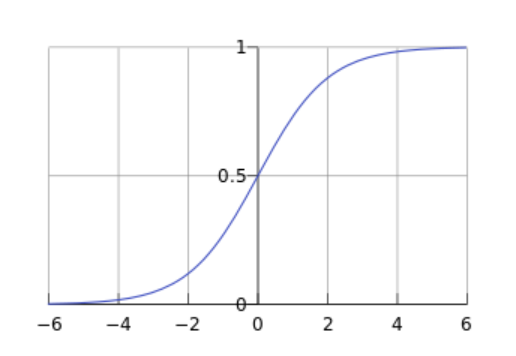
\includegraphics[width=0.6\columnwidth]{4.png}
\end{center}

此函数的意义:以0.5为界,大于0.5被分为“1”类,而小于“0.5”被分为“0”类。将任意的输入数据都映射到(0,1)区间。然后在线性回归中得到一个了预测值,再将该值映射到Sigmoid函数中,这样就完成了由值到概率的转换,实现了分类的目的。

\subparagraph{步骤}:

1) 构建阶跃函数,即Sigmoid函数,将数据进行二分类;

2) 构造代价函数,将模型进行优化处理;

3) 使得代价函数最小并求得回归参数($\theta$)

\subparagraph{模型构建与测试}:

模型中的默认最大迭代次数不够大,这里设置一个最大迭代次数。首先尝试着去设置模型中的一些参数,将训练数据放入模型中训练,然后用测试数据放入训练好的模型中去测试,根据测试结果调整参数,优化模型。

\paragraph{5. 硬投票}.

\subparagraph{简述}

投票法(voting)是集成学习里面针对分类问题的一种结合策略。基本思想是选择所有机器学习算法当中输出最多的那个类。分类的机器学习算法输出有两种类型:一种是直接输出类标签,另外一种是输出类概率,使用前者进行投票叫做硬投票(Majority/Hardvoting),使用后者进行分类叫做软投票(Soft voting)。
sklearn中的VotingClassifier是投票法的实现。在这里,我们采用硬投票的方式。

\subparagraph{模型构建}:

上述三个模型的集成称为“异种集成学习”分类器,将我们训练好的模型传入投票器中,依照“少数服从多数”的规则进行投票,输出预测结果。投票法有较好的模型互补性质,能够将三个模型的预测结果进行综合考量。

\subparagraph{模型保存与加载}:

将上述训练好的模型保存到本地,在进行测试数据预测时,因为我们应事先留好了函数的接口,则只需要加载训练好的模型进行预测即可。

\subsubsection{模型优化}

数据不平衡问题:我们首先采用SMOTE算法,它的基本思想是对少数类样本进行分析并人工合成新样本添加到数据集,但是经过SMOTE算法处理后的数据预测正确率反而降低。因此我们采用朴素随机过采样的方法,将实施高送转的股票比率从15\%提升到30\%,并且经过测试后发现,实施高送转的预测准确率明显上升。

对于“预增预减”和“超涨超跌”两个因子数据,我们在测试时将这两个因子删去后进行模型测试,对预测结果影响较小,因此将这两个因子数据剔除。

\subsubsection{模型评估}

\textbf{优点}:在因子数据的提取中和数据分析中,我们参考了现有的论文资料和经济学原理,根据本题的数据来进行特征值的提取。

在模型的构建上采用硬投票将决策树、KNN和Logistics回归三种算法进行“组合”,形成一种异种集成学习分类器,使得预测准确性保持在80\%左右。

\textbf{缺点}:在分析基础数据时,没有将行业划分和概念板块等特征值进行提取,并且在因子数据“次新股”中,考量不够全面,特别是上市公司在七年前是否为“次新股”这样一个判断中,现有数据没有给出一个很好的标准。在构建决策树中。我们只考虑了树的深度,没有考虑后剪枝的方法进行模型优化。

\subsection{结果分析}

1)在此,我们调用Sklearn的分类报告库,返回分类报告。每次的测试中,投票正确率均在80\%以上。

值得关注的是,在预测上市公司不进行高送转的准确率、精确率和召回率都较为可观,整体在80\%左右。但是预测高转送的准确率、召回率都较低,预测准确率在70\%左右。

对于这样的结果可能原因:一是我们每个模型局部不够“最优”,预测时容易造成过拟合的现象;可用样本(专家样本)中高送转和非高送转的数据样本分布不均衡,经过朴素随机过采样对数据分布有所调整,但并不能完全解决这个问题。因此我们在进行模型机器学习时,模型“较为熟练掌握了不实施高送转的特征”,而学习实施高送转却不尽人意。或许我们可以猜想,与高送转相关的因子可能不止于数据表中的因子,还有一些等待挖掘的因子。


2) 投票正确率: 0.8149

\begin{center}
		\begin{tabular}{|l|l|l|l|l|}
			\hline
			& precision & recall & f1-score & support \\\hline
			0            & 0.83      & 0.96   & 0.89     & 1950    \\\hline
			1            & 0.71      & 0.35   & 0.47     & 595     \\\hline
			accuracy     &           &        & 0.81     & 2545    \\\hline
			macro avg    & 0.77      & 0.65   & 0.68     & 2545    \\\hline
			weighted avg & 0.80      & 0.81   & 0.79     & 2545   \\\hline
		\end{tabular}
\end{center}

\section{结论}

\textbf{针对问题一:}经过数据分析和模型训练,我们发现“超涨超跌”和“预增预减”对于模型的预测准确率并没有明显的影响,因此我们选取的会对高送转产生影响的因子有:

基础因子:股价、总股本、上市年限

成长因子:每股未分配利润、每股资本公积、每股现金流量净额、每股收益、每股净资产、营业总收入同必增长

潜在因子:次新股、近两年送转比率

\textbf{针对问题二:}我们预测以下271支股票在第八年将会进行高送转:
\begin{lstlisting}
[10, 11, 12, 23, 40, 42, 44, 60, 150, 151, 158, 171, 175, 179, 187, 191, 201, 213, 215, 224, 225, 232, 249, 258, 265, 266, 277, 293, 338, 354, 356, 389, 398, 417, 458, 465, 466, 470, 476, 507, 509, 512, 518, 527, 533, 534, 539, 544, 565, 566, 570, 598, 603, 607, 612, 621, 628, 637, 648, 654, 662, 668, 694, 724, 742, 747, 762, 764, 769, 781, 793, 807, 842, 847, 852, 858, 863, 875, 885, 887, 902, 922, 925, 955, 957, 968, 1003, 1013, 1033, 1044, 1064, 1071, 1085, 1101, 1117, 1118, 1142, 1161, 1166, 1181, 1183, 1218, 1242, 1260, 1305, 1321, 1327, 1332, 1346, 1386, 1400, 1429, 1446, 1460, 1506, 1510, 1512, 1524, 1532, 1548, 1555, 1559, 1571, 1588, 1591, 1600, 1607, 1616, 1625, 1639, 1660, 1668, 1690, 1694, 1704, 1731, 1734, 1758, 1759, 1761, 1769, 1771, 1801, 1811, 1817, 1830, 1835, 1839, 1860, 1874, 1886, 1901, 1909, 1922, 1926, 1933, 1946, 1949, 1967, 2024, 2028, 2060, 2079, 2113, 2119, 2124, 2146, 2162, 2182, 2197, 2211, 2225, 2239, 2246, 2247, 2269, 2279, 2300, 2307, 2322, 2330, 2352, 2353, 2366, 2409, 2437, 2438, 2477, 2492, 2505, 2516, 2529, 2533, 2540, 2550, 2552, 2559, 2560, 2593, 2604, 2605, 2630, 2637, 2643, 2652, 2673, 2700, 2703, 2706, 2707, 2724, 2733, 2748, 2759, 2762, 2774, 2807, 2817, 2843, 2881, 2894, 2914, 2918, 2919, 2920, 2932, 2949, 2958, 2961, 2967, 2971, 2977, 2985, 2991, 3009, 3026, 3027, 3038, 3056, 3074, 3112, 3119, 3126, 3127, 3129, 3136, 3188, 3207, 3217, 3220, 3243, 3245, 3257, 3279, 3294, 3295, 3296, 3300, 3309, 3311, 3312, 3341, 3348, 3354, 3356, 3362, 3367, 3376, 3414, 3422, 3445]
\end{lstlisting}



\begin{thebibliography}{5}
	\addcontentsline{toc}{section}{参考文献}
	\bibitem{基于集成学习的上市公司高送转预测模型及投资策略设计}
	胡宸,
	\textit{《基于集成学习的上市公司高送转预测模型及投资策略设计》},
	上海师范大学
	\bibitem{基于模式识别的“高送转”预测模型}
	石 好,
	邢小艳,
	\textit{《基于模式识别的“高送转”预测模型》},
	华南理工大学数学学院,
	广东 广州
	\bibitem{基于集成学习的高送转股票研究}
	王 凯,
	龙卫江,
	\textit{《基于集成学习的高送转股票研究》},
	华南理工大学数学学院,
	广东 广州
	\bibitem{统计学习方法}
	李航,
	\textit{《统计学习方法[M]》},
	北京,
	清华大学出版社,
	2012
	\bibitem{机器学习}
	周志华,
	\textit{《机器学习》},
	清华大学出版社,
	2016
\end{thebibliography}

\end{document}